% Copyright (c) 2012 Raniere Silva <r.gaia.cs@gmail.com>
% Copyright (c) 2012 Fernando Cezarino <feolce@gmail.com>
% Copyright (c) 2012 Ana Paula Diniz Marques <anapdinizm@gmail.com>
% Copyright (c) 2012 Camile Kunz <camileknz@gmail.com>
% Copyright (c) 2012 Ana Flavia <anaflavia.c.lima@gmail.com>
%
% This file is part of 'MS480 - 2012S2 - Aterro com Obstáculo'.
%
% 'MS480 - 2012S2 - Aterro com Obstáculo' is licensed under the Creative
% Commons Attribution-ShareAlike 3.0 Unported License. To view a copy of
% this license, visit http://creativecommons.org/licenses/by-sa/3.0/.
%
% 'MS480 - 2012S2 - Aterro com Obstáculo' is distributed in the hope
% that it will be useful, but WITHOUT ANY WARRANTY; without even the
% implied warranty of MERCHANTABILITY or FITNESS FOR A PARTICULAR
% PURPOSE.

\section{Intersecção de Círculo com Reta} \label{sse:circle_line}
\nocite{Wolfram:CircleLine}
Considere um círculo, $C$, com centro em $(0, 0)$ e raio $r$ e os pontos $P =
(p_1, p_2)$ e $Q = (q_1, q_2)$. A reta $\overline{PQ}$ pode
\begin{itemize}
    \item não interseptar o círculo $C$,
    \item ser tagente ao círculo $C$, ou
    \item ter dois pontos em comum com o círculo $C$,
\end{itemize}
como ilustrado na Figura~\ref{fig:circle_line}.
\begin{figure}[!htb]
    \centering
    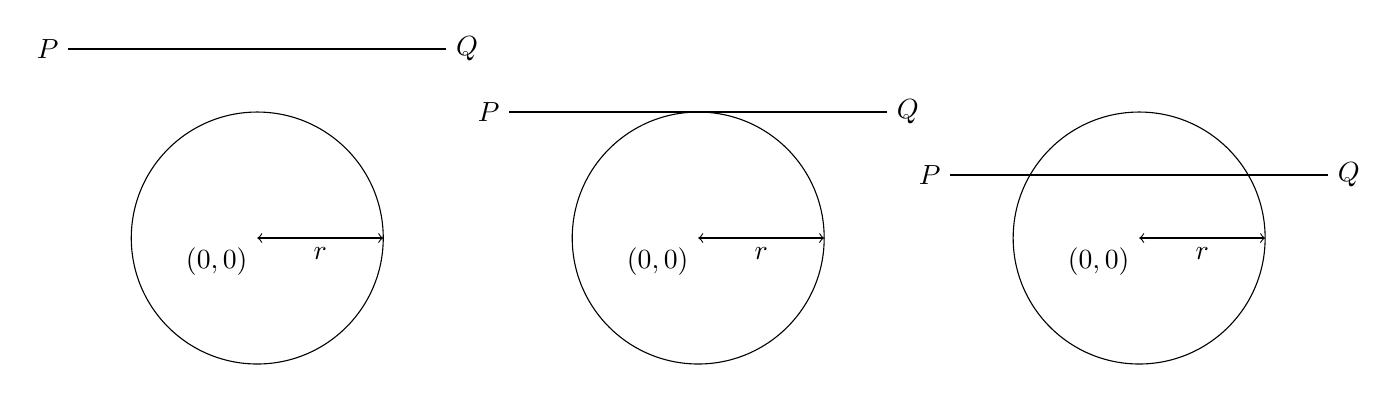
\begin{tikzpicture}[scale=0.8]
        \draw (0,0) circle (2);
        \draw[<->] (0,0) node[below left]{$(0, 0)$} -- +(2, 0)
        node[midway, below]{$r$};
        \draw (-3,3) node[left]{$P$} -- (3,3) node[right]{$Q$};
        \draw (7,0) circle (2);
        \draw[<->] (7,0) node[below left]{$(0, 0)$} -- +(2, 0)
        node[midway, below]{$r$};
        \draw (4,2) node[left]{$P$} -- (10,2) node[right]{$Q$};
        \draw (14,0) circle (2);
        \draw[<->] (14,0) node[below left]{$(0, 0)$} -- +(2, 0)
        node[midway, below]{$r$};
        \draw (11,1) node[left]{$P$} -- (17,1) node[right]{$Q$};
    \end{tikzpicture}
    \caption{Possíveis interseção de um círculo e uma reta. A interseção é
    vazia na figura a esquerda, a interseção corresponde a um único ponto na
    figura no centro e a interseção corresponde a dois pontos distintos na
    figura a direita.}
    \label{fig:circle_line}
\end{figure}

A equação do círculo é
\begin{align}
    x^2 + y^2 &= r^2
    \label{ec_circ}
\end{align}
e a equação da reta que passa pelos pontos $P$ e $Q$ é
\begin{align*}
    (y-p_2)(q_1-p_1)=(q_2-p_2)(x-p_1)\,.
\end{align*}
Se $p_1\neq q_1$, esta equação pode ser escrita como
\begin{align*}
    y=(x-p_1)\left(\frac{q_2-p_2}{q_1-p_1}\right)+p_2\,,
\end{align*}
ou ainda
\begin{align*}
    y = x\left( \frac{q_2 - p_2}{q_1 - p_1} \right) + \left(
    \frac{q_1 p_2 - q_2 p_1}{q_1 - p_1} \right).
\end{align*}

Substituíndo em (\ref{ec_circ}), obtemos
\begin{align*}
    x^2  + \left[ \left( \frac{q_2 - p_2}{q_1 - p_1} \right) x + \left(
    \frac{q_1 p_2 - q_2 p_1}{q_1 - p_1} \right) \right]^2  = r^2\,,
\end{align*}
ou ainda
\begin{align*}
    \left[ 1 + \left( \frac{q_2 - p_2}{q_1 - p_1} \right)^2 \right] x^2 +
    2 \left( \frac{q_2 - p_2}{q_1 - p_1} \right) \left( \frac{q_1 p_2 - q_2
    p_1}{q_1 - p_1} \right) x + \left( 
    \frac{q_1 p_2 - q_2 p_1}{q_1 - p_1} \right)^2 & = r^2\,.
\end{align*}
Para a equação do segundo grau anterior, o discriminate é
\begin{align*}
    \Delta &= r^2 \left( \left( q_1 - p_1 \right)^2 + \left( q_2 - p_2
    \right)^2 \right) - \left( p_1 q_2 - p_2 q_1 \right)^2\,;
\end{align*}
e
\begin{itemize}
    \item se $\Delta < 0$ a equação não possui solução real,
    \item se $\Delta = 0$ a equação possui duas soluções reais iguais,
    \item se $\Delta > 0$ a equação possui duas soluções reais distintas.
\end{itemize}
Logo,
\begin{itemize}
    \item $\overline{PQ}$ não interseptar o círculo $C$ quando $\Delta < 0$,
    \item $\overline{PQ}$ é tagente ao círculo $C$ quando $\Delta = 0$,
    \item $\overline{PQ}$ tem dois pontos em comum com o círculo $C$ quando
        $\Delta > 0$.
\end{itemize}
